\documentclass{scrreprt}
\usepackage[ngerman]{babel}
\usepackage[utf8]{inputenc}
\usepackage{graphicx}

\begin{document}
	\chapter*{Spiel}
	Idee:
	\begin{itemize}
		\item kleines Rollenspiel mit einfacher Grafik
		\item Kartenspiel als Minispiel, da es keine Kampfanimationen gibt
		\item NPC sollen die Karte bevölkern
	\end{itemize}

	\section*{5.9.}
	\begin{itemize}
		\item Fenster öffnen
		\item Karte laden und anzeigen
	\end{itemize}

	\section*{8.9.}
	\begin{itemize}
		\item Laptop vergessen $\leftarrow$ Ideen weiterentwickeln
		\item Karte angepasst
		\item neue Sprites für die Figuren gesucht
		\item Minispiel entwickelt
		\item Geschichte erstellt
	\end{itemize}

	\section*{12.9.}
	\begin{itemize}
		\item Rendercode angepasst
		\item Charakteranimationen hinzugefügt
	\end{itemize}

	\section*{15.9.}
	\begin{itemize}
		\item Bäume können einfacher erstellt werden
		\item mehrere Charaktere werden unterstützt
	\end{itemize}

	\section*{19.9.}
	\begin{itemize}
		\item Dialoge eingefügt (aus JSON-Datei geladen)
		\item Anleitung eingefügt
	\end{itemize}

	\section*{22.9.}
	\begin{itemize}
		\item Wegfindung implantiert (Breitensuche)
		\item Häuser eingefügt4
	\end{itemize}

	\section*{26.9.}
	\begin{itemize}
		\item Minispiel angefangen
		\item Wegfindung verbessert (A-Stern)
	\end{itemize}

	\section*{6.10.}
	\begin{itemize}
		\item Minispiel fertiggestellt
		\item Endgegner hinzugefügt
	\end{itemize}

	\section*{Anleitung}
	Spiel starten und die Einweisung startet automatisch. Für das Kartenspiel: Eichel ist höher als Blatt, Blatt ist höher als Rot, Rot ist höher als Schellen. Ass ist höher als König, König als Ober, Ober als Unter, Unter als 10, 10 als 9, 9 als 8, 8 als 7.
	
	\begin{figure}
		\centering
		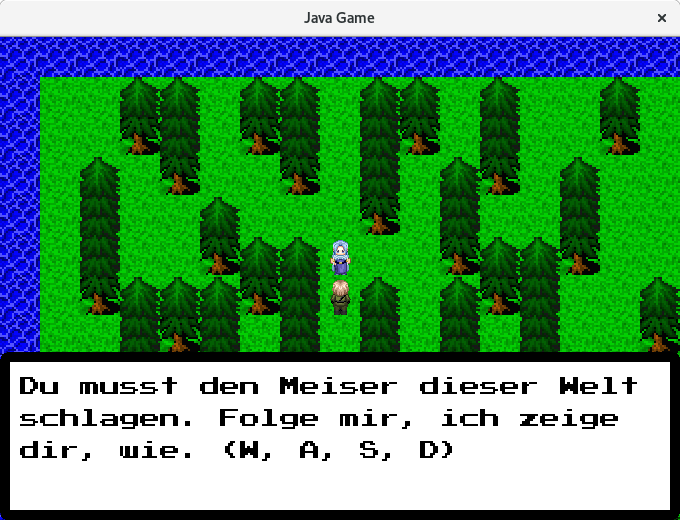
\includegraphics[width=0.5\textwidth]{ingame.png}
		\caption{Der Anfang des Spiels mit Anleitung}
	\end{figure}

	\begin{figure}
		\centering
		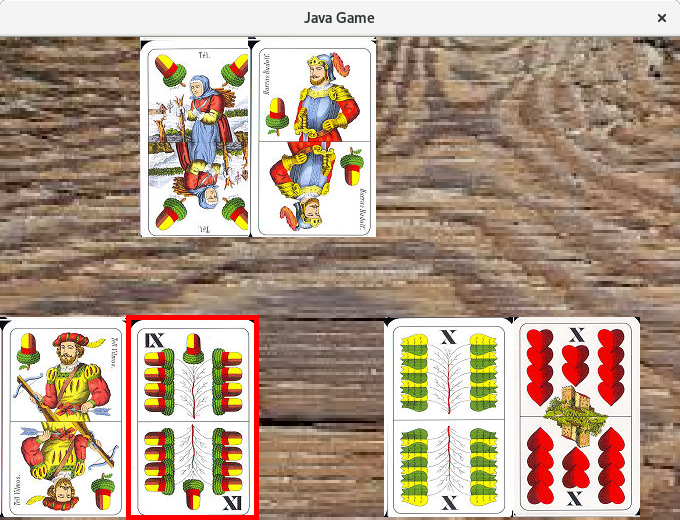
\includegraphics[width=0.5\textwidth]{mini.png}
		\caption{Das Minispiel}
	\end{figure}
\end{document}